%!TEX root = ../main.tex
% Chapter 8

\chapter{Technische Konzeption des Systems}
\label{Technische_Konzeption_des_Systems}

Dieses Kapitel beschäftigt sich mit der technischen Konzeption des Systems, wobei die Erkenntnisse der Markt- und Forschungsrecherche aus Kapitel \ref{Erkenntnisse_fuer_das_zu_entwickelnde_System} als Basis für die Architektur dienen. Modelliert wird diese Architektur mit einem Datenmodell und einem Komponentenmodell, anhand welchem eine geeignete Programmiersprache, ggf. mit entsprechenden Pattern, ausgewählt wird.

Die für die Entwicklung relevanten Funktionen können in drei Module unterteilt werden: Erweiterung des Absender-Clients, Empfänger-Client und Zahlungsmodul. Die Erweiterung des Absender-Clients beschreibt Plugins, die unterschiedliche E-Mail Clients erweitern. Da hierfür keine universelle Anwendung geschaffen werden kann, wird ein Web-Frontend implementiert, welches von verschiedenen Clients dargestellt werden kann. Innerhalb des Frontends wird das Headerfeld generiert, welches der Nutzer daraufhin in seinem Client hinterlegen kann. Der Empfänger-Client ist eine neu zu entwickelnde Anwendung, die sowohl ein Backend zur Speicherung der priorisierten E-Mails, als auch ein Frontend zur Darstellung jener benötigt. Das Zahlungsmodul ist ein Backend, welches die Zahlungen verwaltet und speichert. Es wird sowohl vom Absender-Frontend, als auch von der Anwendung des Empfängers kontaktiert. Darüber hinaus verwaltet es die Token, die jedem Nutzer zur Verfügung stehen.

\section{Datenmodell}
\label{Datenmodell}
Die Systemarchitektur versucht im ersten Schritt das Content Model aus Kapitel \ref{Content_Model} in ein sprachunabhängiges Datenmodell zu überführen. Das Modell orientiert sich dabei an objektorientierten Strukturen. Sollte eine Sprache ausgewählt werden, die keine Objekte oder Datentypen unterstützt, dient das Datenmodell als inhaltlicher Leitfaden zum Aufbau der einzelnen Variablen. Im Gegensatz zu UML wird auf die Definition von Methoden verzichtet, da sich das Datenmodell auf Objekte bezieht, die in der Datenbank abgelegt werden, was nicht dem vollen Umfang der Anwendung entspricht. Das Modell ist in Abbildung \ref{fig:Datenmodell} zu sehen.

Die \texttt{Message} repräsentiert eine E-Mail und enthält alle aus dem Content Model bekannten Felder, die auch den E-Mail Headern entsprechen. Da diese per Definition Key-Value-Paare sind, können sie als Strings typisiert werden. Als ID wird, wie bei den anderen Objekten auch, eine \textit{UUID} verwendet. UUIDs sind generierte 128 Bit-Nummern, die in RFC 4122 definiert wurden. Der Vorteil ist, dass die Wahrscheinlichkeit eines Duplikates äußerst gering und in der Anwendung zu vernachlässigen ist \citep[S. 2]{RFC4122}. Im Modell werden sie als eigener Datentyp aufgeführt, je nach Programmsprache werden sie unter Umständen als String gespeichert. Die Anhänge der E-Mail sind als Datei definiert, auch hier stellt sich die Frage, inwiefern die Sprache einen solchen Datentyp unterstützt. Außerdem enthält die E-Mail den Gegenwert, in Form eines \texttt{Value}. Zusätzlich zu seiner UUID und der Menge des Wertes enthält er die E-Mail Adressen des Absenders und Empfängers, sowie den Zeitpunkt der E-Mail. Diese Informationen sind bewusst redundant gehalten, um nicht nur den E-Mail Header, also die UUID des Gegenwertes, sondern weitere Felder abzugleichen. Somit wird verhindert, dass ein Gegenwert-Header mehrfach verwendet wird, da er an Absender, Empfänger und Zeitpunkt geknüpft ist.

Das zentrale Objekt der Anwendung ist der Posteingang, die \texttt{Inbox}. Sie existiert für jeden registrierten Empfänger und enthält die E-Mails, Informationen zum Empfänger, sowie Sonderregeln. Der Empfänger wird mit UUID, Name, E-Mail Adresse, Anmeldeinformationen, sowie Bearbeitungsleistung hinterlegt. Letztere wird als numerischer Wert pro Tag definiert und ist für Absender sichtbar. Die Sonderregeln sind optional und können beliebig oft angelegt werden. Sie bestehen aus der UUID, dem \texttt{field\_to\_search} und dem \texttt{field\_matcher}. Ersteres definiert in welchen Headern eine Bedingung gelten muss, Zweiteres definiert welche Bedingung gelten muss. So kann der Betreff der E-Mail ein mögliches \texttt{field\_to\_search} und der Text \textit{Wichtig} ein möglicher \texttt{field\_matcher} sein.

\begin{figure}[!ht]
	\centering
		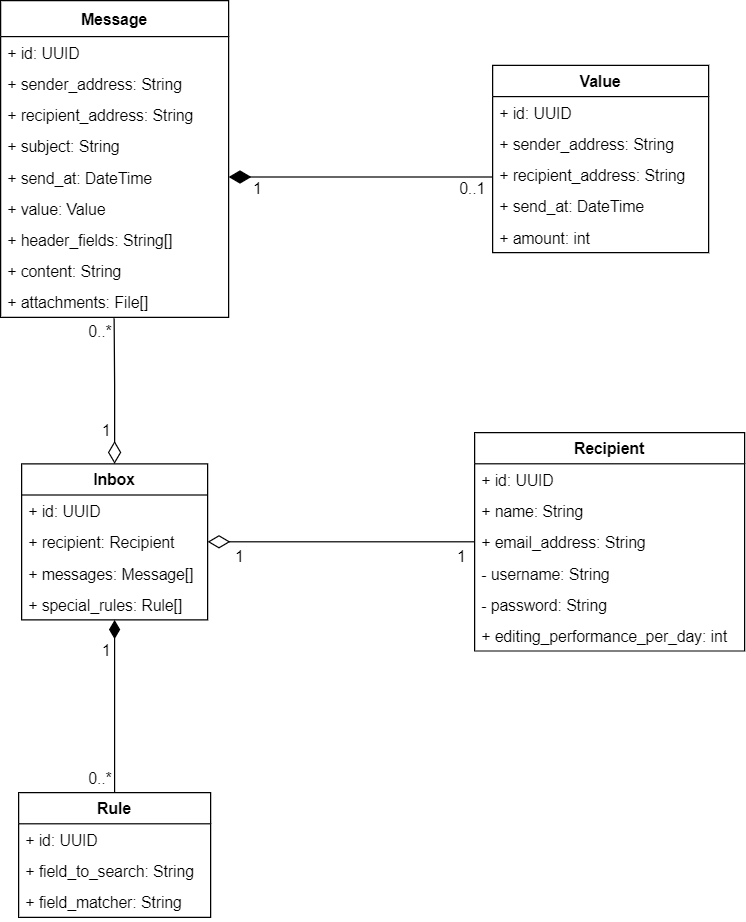
\includegraphics[width=1\textwidth]{Figures/Datenmodell.png}
	\caption{Datenmodell, angelehnt an UML}
	\label{fig:Datenmodell}
\end{figure}

% --------------------------------------------------------------------

\section{Komponentenmodell}
\label{Komponentendiagramm}
Im Gegensatz zum Datenmodell versucht das Komponentenmodell die gesamte Systemarchitektur abzubilden. Der Fokus liegt auf den Bestandteilen des Systems, sowie der Protokolle, mit welchen sie kommunizieren. Die in den Komponenten enthaltene Anwendungslogik wird in Kapitel \ref{Implementation_des_Systems} detailliert erläutert. Das Komponentenmodell ist nach \acrfull{mvc} aufgebaut. MVC ist ein Pattern, nach welchem die Daten (\textit{Model}), das UI (\textit{View}) und die Anwendungslogik, beziehungsweise die HTTP-Routen (\textit{Controller}) getrennt werden. Das Komponentenmodell in Abbildung \ref{fig:Komponentenmodell} zeigt die Teile des Pattern in verschiedenen Farben.

\begin{figure}[!ht]
    \centering
 	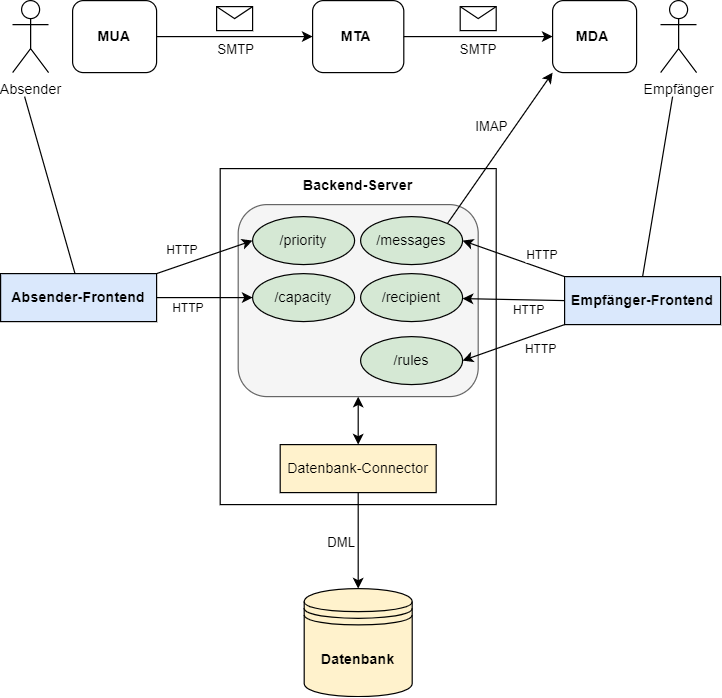
\includegraphics[width=1\textwidth]{Figures/Komponentenmodell.png}
	\caption{Komponentenmodell mit Model (gelb), View (blau) und Controller (grün)}
	\label{fig:Komponentenmodell}
\end{figure}

\noindent Die Interaktion mit dem System beginnt beim Absender, der das Absender-Frontend aufruft. Das Frontend ruft das aktuelle Aufkommen des Empfängers mit \texttt{GET /capacity} oder die zur Priorisierung notwendigen Token/Beträge mit \texttt{GET /priority} auf. Entscheidet sich der Absender seine E-Mail priorisieren zu wollen, wählt er dies im Absender-Frontend aus, sodass die Priorisierung mit \texttt{POST /priority} an das Backend weitergeleitet wird. Die Controller rufen die entsprechenden Daten von der Datenbank ab. Je nach Sprache ist ein Datenbank-Connector zwischengeschaltet. Die Kommunikation mit der Datenbank wird über eine \acrfull{dml} realisiert.

Nach dem Erhalt des Header-Feldes formuliert der Absender die E-Mail in seinem MUA und versendet sie herkömmlich über SMTP. Im Gegensatz zum ursprünglichen Prozess ruft der Empfänger seine E-Mails nicht über seinen MUA ab. Stattdessen öffnet er das Empfänger-Frontend, welches die E-Mails über IMAP von seinem MDA abruft und anzeigt. Dafür wird \texttt{GET /messages} im Backend aufgerufen. Nach dem Abrufen der Nachrichten sortiert das Frontend automatisch. Zusätzlich wird über \texttt{GET /rules} geprüft inwieweit Nachrichten außerhalb ihrer Priorität vorgezogen werden müssen. Der Empfänger hat die Möglichkeit diese Regeln selbstständig anzupassen, dabei wird das Backend mit \texttt{PUT /rules} angesprochen. Selbiges gilt beim Bearbeiten/Abrufen der Empfängerinformationen, wie z.B. der Bearbeitungsleistung. Hierfür nutzt das Frontend die Ressource \texttt{/recipient}.

Das Versenden von Antworten wird im Kontext dieser Arbeit nicht behandelt, würde jedoch auch über das Empfänger-Frontend realisiert werden. Hierbei wäre zu klären, ob dafür der Backend-Server verwendet wird oder ob das Frontend die Nachrichten direkt über SMTP versendet.

% --------------------------------------------------------------------

\section{Auswahl der Programmiersprache und Pattern}
\label{Auswahl_der_Technologie_und_Designpattern}

Im Folgenden sollen die zu verwendenden Sprachen und Software Pattern definiert und beschrieben werden. Hierbei wird versucht möglichst wenige Sprachen zu nutzen, um die Entwicklungszeit zu minimieren. Die Auswahl eines Patterns hängt von der Sprache ab. So definieren manche Sprachen ein Pattern vor (diese werden auch \emph{opinionated languages} genannt), während andere die Entscheidung beim Entwickler belassen.

\subsection{Node.js}
\label{Node.js}

\textit{Node.js} ist eine Laufzeitumgebung, welche es ermöglicht JavaScript außerhalb des Browsers und somit serverseitig auszuführen. Die Software ist Open Source und wurde 2009 von Ryan Dahl entwickelt, später von der OpenJS Foundation übernommen. Im Gegensatz zu im Browser ausgeführtem JavaScript ist Node.js asynchron, sodass lang laufende Operationen, wie Requests an andere Server oder das Warten auf Input nicht das gesamte System blockieren, sondern mit Callbacks bearbeitet werden. Durch diese Asynchronität sind Node.js Anwendungen einfach skalierbar und können auch große Lasten bewältigen. Hinzu kommt, dass Node.js eventbasiert funktioniert. Das bedeutet, dass ein Server auf Requests, in diesem Fall das Event, von einem Client wartet und darauf aufbauend Anwendungslogik ausführt. Dadurch wird die Implementation von REST-konformen Anwendungen ermöglicht. \citep{OpenJSFoundation2022}

In der ursprünglichen Version von Node.js ist eine kleine Anzahl von Modulen enthalten, die Standardfunktionalitäten abdecken soll. Zu diesen gehören unter anderem seit Version 18 die \texttt{fetch API}, die HTTP/S-Requests ermöglicht und das Modul \texttt{fs}, mit welchem Zugriffe auf das Dateisystem möglich sind. Auch das Erzeugen von mehreren Kindprozessen ist mit \texttt{child\_process.fork} möglich. Für Serveranwendungen ist das HTTP-Modul relevant, mit welchem HTTP-Server, Ressourcen und Listener auf verschiedene HTTP-Methoden wie \texttt{GET} oder \texttt{POST} erstellt werden können. Darüber hinaus lässt sich Node.js mit zahlreichen Modulen erweitern, die zum Beispiel auf der Plattform \texttt{npmjs.org} veröffentlicht werden. Diese in JavaScript geschriebenen Plugins können Node.js um zahlreiche Funktionalitäten, wie WebSockets, Anbindung an Cloud Services über SDKs, Tests etc. erweitern.

Die leichtgewichtige Struktur von Node.js bringt Vorteile für die Entwicklung von Pay2Mail mit sich. So können Module und Abhängigkeiten gezielt importiert werden wodurch die Größe des Servercodes minimal bleibt. Darüber hinaus kann die Systemarchitektur frei gewählt und konstruiert werden. Durch die Bekanntheit von Node.js gibt es zudem zahlreiche Hostinganbieter, bei denen sich eine Anwendung ohne eine große Konfiguration oder Installation betreiben lässt. Dadurch lassen sich auch CI/CD-Pipelines etablieren, die die Anwendung beispielsweise bei einem Cloud-Anbieter wie \acrfull{aws} veröffentlichen.

Ein Nachteil von Node.js ist, dass es keine vorgegebenen Designpattern oder Prinzipien gibt, nach welchen eine Anwendung implementiert werden muss. So ist es mit Node.js, wie mit JavaScript allgemein, möglich Anwendungen zu schreiben, die Antipattern enthalten oder anfällig für Fehler sind. Zwar gibt es Analysetools für JavaScript, wie z.B. ESLint, allerdings sind diese meist auf Syntax beschränkt und können keine Systemarchitektur analysieren und bewerten. Hinzu kommt, dass Entwickler für diverse Funktionalitäten externe Module brauchen. Zwar macht dies das Framework flexibel, sorgt aber dafür, dass stabile Module gefunden, aktuell gehalten und erlernt werden müssen. Versuchen neue Entwickler sich in die Software einzuarbeiten, müssen sie nicht nur mit Node.js, sondern auch mit der Funktionsweise diverser Module vertraut sein. Im Falle von Pay2Mail bedeutet das, dass eine Datenbank separat gehostet werden muss, zudem muss ein entsprechender Connector geschrieben oder als Modul eingebunden werden. Beim Frontend bietet Node.js ebenfalls keine Templatesprache, sodass vom Server gerenderte Seiten (auch Server Site Rendering (SSR) genannt) nur über ein Modul oder ein Framework wie Astro oder Nuxt.js zu realisieren sind. Die Notwendigkeit für Pay2Mail zahlreiche Module zu importieren und somit die Stabilität des Systems zu gefährden (siehe Anforderung \textit{Integrität der E-Mails und Zahlungen} in Kapitel \ref{Anforderungen_von_Empfaengern}) bedeutet, dass sich Node.js nicht für die Entwicklung des Systems eignet.

\subsection{Laravel}
\label{Laravel}

\textit{Laravel} ist ein von Taylor Otwell im Jahr 2011 entwickeltes Framework, welches auf PHP aufbaut. Es bietet die Möglichkeit Anwendungen nach dem \textit{\acrfull{mvc}}-Pattern zu implementieren. Es zeichnet sich dadurch aus, dass es als Fullstack Framework genutzt werden kann. Das bedeutet, dass es Funktionalitäten für Datenbanken, APIs, Frontends und Authentifizierung enthält. Dadurch ist es möglich vollumfängliche Webanwendungen zu implementieren, ohne auf Module von Drittanbietern zurückgreifen zu müssen. Darüber hinaus bietet Laravel nativ die Möglichkeit die Anwendungen mit Docker in Container zu verpacken und so einfacher zu deployen. Auch die Skalierbarkeit ist ein Kernaspekt, mit welchem es möglich ist Anwendungen zu entwickeln, die große Lasten tragen können \citep{Otwell2022}.

Das opinionated MVC-Pattern ist ein Vorteil, da es Entwickler dazu zwingt ihre Anwendungen zu strukturieren und bereits vor der Implementation zu wissen, welche Anforderungen sie wie erfüllen wollen. Im Falle von Pay2Mail hilft es zusammen mit der integrierten Datenbank das Content Model aus Kapitel \ref{Content_Model} mit möglichst wenig Abweichungen implementieren zu können. Da für den Empfänger eine Authentifizierung notwendig ist, ist es von Vorteil, dass Laravel diese direkt mit sich bringt.

Ein großer Nachteil von Laravel ist die Lernkurve, die insbesondere zu Beginn recht steil ist. Während das für große Systeme, die Produktionsreife erreichen sollen, kein Hindernis darstellt, sorgt es bei Pay2Mail dafür, dass die Entwicklung des ersten Prototyps stark verzögert wird. Ein weiteres Problem ist darunter liegende Sprache PHP, die keine festen Datentypen hat. Das hat zur Folge, dass Anwendungen weniger performant sind, Fehler aufgrund von falsch genutzten Variablen entstehen und die Fehleranalyse deutlich zeitintensiver ist. Da Pay2Mail nach den Anforderungen in Kapitel \ref{Anforderungen_von_Absendern} die Bearbeitung von E-Mails nicht einschränken oder verlangsamen soll, eignet sich Laravel nicht zur Implementation des Systems.


\subsection{Ruby on Rails}
\label{Ruby_on_Rails}

\textit{Ruby on Rails} (auch kurz \textit{Rails}) ist ein ursprünglich von David Heinemeier Hansson entwickeltes Framework auf Basis der Sprache Ruby. Wie Laravel basiert es auf MVC und ist ein opinionated Fullstack Framework. Es unterscheidet sich jedoch dadurch, dass es von zwei grundlegenden Prinzipien getragen wird: \textit{Don't Repeat Yourself (DRY)} und \textit{Convention Over Configuration}. DRY bedeutet, dass nach Möglichkeit kein Code dupliziert werden soll. Existieren beispielsweise jeweils Datenmodelle für ein Haus und eine Wohnung, die sich zu 90\% ähneln, sollen diese nicht getrennt formuliert werden. Stattdessen sollen sie von einer Klasse, beispielsweise Gebäude erben, um nur noch ihre für sich spezifischen Eigenschaften zu definieren. Dieses Prinzip kommt auch bei der Erstellung von HTTP-Ressourcen oder Views zu tragen. So empfiehlt Rails beispielsweise wiederkehrende UI-Elemente in \textit{Partials} zu auszulagern und sie an verschiedenen Stellen aufzurufen. Das Prinzip Convention Over Configuration beschreibt den Ansatz, nach welche Rails viele Konfigurationen nicht zwingend benötigt, sondern stattdessen Standardwerte und -verhalten definiert, die für den Großteil der Entwickler eine nutzbare Basis bilden. Diese Standards werden auch \textit{reasonable defaults} genannt und sind für die meisten Aufrufe innerhalb des Frameworks vorhanden \citep{Hansson2022a}.

Ruby on Rails bringt eine Vielzahl von Funktionalitäten mit sich, z.B. eine integrierte Datenbank mit dem Modul \textit{Active Record} zur Abstraktion, Internationalisierung mit \textit{I18N} und eine Testumgebung, die Unit Tests, Integration Tests und End to End Tests ermöglicht. Das Rendern von Views wird mit \acrfull{erb} ermöglicht. Ähnlich wie in PHP können HTML-Dokumente um Passagen in Ruby erweitert werden, wo notwendig. So können Instanzvariablen aus dem Controller an eine View weitergegeben und serverseitig verwendet werden. Zusätzlich können JavaScript-Frameworks wie Vue.js, React oder Svelte im Frontend verwendet werden, wobei das Framework \textit{Hotwire} standardmäßig verfügbar ist. Ein weiterer Vorteil ist das Caching von generierten Seiten, wodurch die Last des Server verringert und somit die Skalierbarkeit verbessert wird.

Der große Vorteil von Ruby on Rails für Pay2Mail ist, dass ein Großteil der Funktionen direkt im Framework enthalten sind und nativ genutzt werden können. Die Templatesprache ERB bietet außerdem die Möglichkeit Seiten direkt an den Client auszuliefern, ohne dass Frontend-seitiges Nachladen von Inhalten notwendig ist. Somit ist die Nutzung eines JavaScript-Frameworks optional, was sich positiv auf die Performance der Anwendung auswirkt und die Verlangsamung des E-Mail Prozesses ausschließt (siehe Kapitel \ref{Anforderungen_von_Absendern}). Auch kann die geforderte Sicherheit der Zahlungen und E-Mails sichergestellt werden. Ruby on Rails ist gegen Session Hijacking, Injections und \acrfull{csrf} abgesichert und bietet darüber hinaus die Möglichkeit weitere Sicherheitsmaßnahmen zu konfigurieren \citep{Hansson2022}. Durch die Prinzipien DRY und Convention Over Configuration ist es im Vergleich zu Laravel und Node.js möglich in kurzer Zeit einen Prototypen zu entwickeln und ihn daraufhin in eine produktions-bereite Anwendung zu erweitern.

Der einzige für das System relevante Nachteil ist, dass eine Authentifizierung nicht im Standard enthalten ist und als externes Modul (auch \textit{Gem} genannt) importiert werden muss. Beliebte Gems für diesen Anwendungsfall sind \textit{devise} oder \textit{authlogic}. Da außerhalb dieses Moduls Ruby on Rails alle Funktionalitäten mitbringt, die für Pay2Mail notwendig sind, wird es für die Entwicklung des Systems ausgewählt. Zur Verbesserung der Performance wird auf ein JavaScript-Framework im Frontend vorerst verzichtet. Falls notwendig, wird Hotwire oder ein anderes leichtgewichtiges Framework eingebunden; das zugehörige Vorgehen wird in Kapitel \ref{Implementation_des_Systems} erläutert.